\chapter{Unmaintainability Factors}
\label{ch:unmaintainability}

As previous work related to the integration of \acrshort{vtk} with external environments already exist, we analyse some of the closest researches to our project to determine which factors cause maintainability issues. Furthermore, we also perform a quick analysis of both \acrshort{vtk} and Unity interfaces to determine what areas of these libraries are the most subject to changes in the interface. Our objective is to determine which factors contribute most to maintainability related issues and design solutions to limit their influence on our software.

As such, we start with the analysis of the libraries' interfaces, focusing mostly on \acrshort{vtk} as we found that it is the most tightly coupled to our software and the cause of most issues of the two. Secondly, we analyse a series of theses produced by the \acrshort{uva} focusing on similar projects as ours \cite{dreuning_visual_2016, shutte_virtual_2018, kruis_creating_2017} and the Wheeler et al. project called VtkToUnity focused on integrating \acrshort{vtk} with Unity to produce a volume rendering software \cite{wheeler_virtual_2018}.

\section{VTK}
\label{ch:unmaintainability-vtk}

As our prime visualization and rendering library, \acrshort{vtk} is widely used in our project. The library presents thousands of classes which range in functionality to data sources, manipulators and filters, rendering, mathematical support, parallelization and distribution support. To study the factors that contribute to our project's maintainability issues, we study the documentation of the library comparing versions 7\footnote{\url{https://vtk.org/doc/release/7.0/html/}} and 9\footnote{\url{https://vtk.org/doc/nightly/html/index.html}} and determine how variable the interface is and whether the library is backwards compatible. We also determine how the API changes and how the modules are distributed, as to see how the building system will be affected.

From the FAQ statement of the \acrshort{vtk} wiki\footnote{\url{https://vtk.org/Wiki/VTK/FAQ\#:~:text=Between\%20regular\%20releases\%20maintain\%20backwards\%20compatibility\%20to\%20the\%20API\%20with\%20prior\%20releases\%20of\%20VTK\%20when\%20doing\%20so\%20does\%20not\%20increase\%20the\%20complexity\%20or\%20readability\%20of\%20the\%20current\%20VTK\%20or\%20when\%20the\%20benefits\%20of\%20breaking\%20the\%20API\%20are\%20negligible.}}, the developers of the library aim at keeping the versions backwards compatible. This being said, there are cases, as highlighted by the same document, in which this compatibility is not guaranteed, especially since version 6 as the backwards compatibility layer between versions 5 and 4 has been removed\footnote{\url{https://vtk.org/Wiki/VTK/VTK_6_Migration/Overview\#:~:text=Overview\%20of\%20Changes,-The\%20changes\%20introduced&text=Removal\%20of\%20VTK\%204\%20backwards\%20compatibility\%20superclasses\%3A\%20This\%20includes\%20vtkProcessObject,order\%20to\%20provide\%20backwards\%20compatibility.}}.

From our evaluation of the library's documentation, we find cases in which API interfaces have changed, e.g in the \verb|vtkOpenGLRenderer| class the \verb|GetPass()| method has been removed and the \verb|DeviceRender()| methods now take a parameter. This being said, such interfaces are made so that they are still backwards compatible, as for the first change the \verb|vtkRenderer| superclass now implements the method and for the second the parameter has a default value of \verb|nullptr| and thus the method can still be called without parameters, making the code backwards compatible. The other instances we find of API changes follow this pattern, thus we believe they are not a big contributing factor to unmaintainability.

What is apparent though is that the library grows fast, and code is continuously shifted, as within minor versions of the same release we can see modules changing: from the versions 8.1 and 8.2, modules such as \verb|vtkm| and \verb|vtkpegtl| are no more present or possibly renamed/moved, a number of new modules created and, as stated in the official changelog of the library, macros removed as the library became C++11 compliant, harming backwards compatibility\footnote{\url{https://blog.kitware.com/vtk-8-2-0/}.}. These changes make it harder to create a shared building system as well as harming general approaches over different versions as changes to the library may break our solution. We believe these to be mild contributing factors to the unmaintainability of solutions built on \acrshort{vtk}.

\begin{figure}
    \centering
    \begin{subfigure}{.45\textwidth}
        \centering
        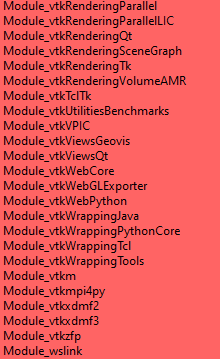
\includegraphics[width=.7\linewidth]{pictures/Vtk-8.1.0-modules-cmake.PNG}
        \caption{Version 8.1}
        \label{fig:sub1}
    \end{subfigure}
    \begin{subfigure}{.45\textwidth}
        \centering
        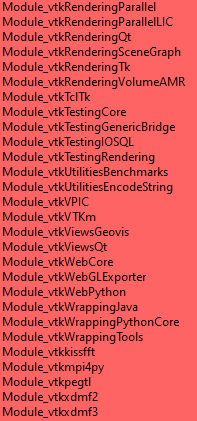
\includegraphics[width=.7\linewidth]{pictures/Vtk-8.2.0-modules-cmake.PNG}
        \caption{Version 8.2}
        \label{fig:sub2}
    \end{subfigure}
    \caption{VTK module comparison between minor versions, taken from the last few of the list}
    \label{fig:vtk-module-comp}
\end{figure}

The biggest factor we find contributing to maintainability issues with \acrshort{vtk} is building the library. During the research and development of our solution, we have found multiple issues with the usage of CMake, a C/C++ cross-platform project building system\footnote{\url{https://cmake.org/}.}, and the building and installation of the Python wrapper of \acrshort{vtk}. The documentation on part of the library is lacking, especially for troubleshooting when issues arise.

In particular, there is little information on how to build and install the \acrshort{vtk} Python wrapper on a Windows system, at least for the latest versions of the library, and we have been unable to use the library in Python with our own built library. Due to this, we were not able to build our own Python wrapper and we used a pre-compiled binary version\footnote{Available at \url{https://www.lfd.uci.edu/~gohlke/pythonlibs/\#vtk}.}.

This issue is mildly mitigated by the active community around the library that can offer support, though this still constitutes an obstacle towards effective building, installation and troubleshooting when working with the library.

%Depending on your subject, you might need multiple research chapters. Moreover, depending on how the research questions are linked, you may need to answer them one by one and then connect the answers into a final discussion chapter. 

%See Canvas for examples of theses with various approaches to structuring the research content.